% This is LLNCS.DOC the documentation file of
% the LaTeX2e class from Springer-Verlag
% for Lecture Notes in Computer Science, version 2.4

\documentclass{llncs}
\usepackage{llncsdoc}
\usepackage{graphicx}
\usepackage{graphics}

\usepackage{pgfplots}
\usepackage[utf8]{inputenc}
\newtheorem{cnj}{Conjecture}

\usepackage{amsmath}
\usepackage[utf8]{inputenc}
%
\begin{document}

\title{Cyber-insurance \& endogenous network formation}

\author{Håvard Råmundal Halse\inst{1}, Jonas Hoemsnes\inst{1} \and Gergely Biczók\inst{2}}

\institute{Dept. of Telematics \\
Norwegian University of Science and Technology \\ \{havahals, jonashoe\}@stud.ntnu.no
\and
Dept. of Telematics \\
Norwegian University of Science and Technology \\ gbiczok@item.ntnu.no}

\maketitle
%

\begin{abstract}
This paragraph shall summarize the contents of the paper
in short terms.
\end{abstract}
%

\section{Modeling Cyber-insurance}
\section{Models}
There are many examples of nodes that need to establish connections with eachother.
For example, when a firm is outsourcing tasks, cooperating or depending on other
firms in some way. Such scenarios could be modeled, as networks where the nodes
represents the firms and the links between them are their dependencies. However,
the link between nodes involves some risks, such as: will the company deliver at the
reported time, to the reported costs, what happens if it fails to deliver, what if the
company goes bankrupt etc. To handle these risks, we need cyber-insurance.

From the insurer’s point of view, a problem with cyber-insurance is to define and calculate risk, because the network structure is
undefined. If an insurer were able to predict the network structure, the calculations
of overall risk would be realizable. The situation could be even better if the insurer
could force the structures found earlier to evolve, hence, ensuring a higher
total payoff for the network. In summary, star topologies, or
star-like topologies, have a fixation probability that exceeds the fixation probability
of circulation graphs. Star structures also have a desirable property of minimizing the
average path length, i.e. minimizing the cost spent on establishing links. Finally, the
clique has a nice property of being able to achieve super-critical payoff, as showed in
[Blu11]--fix. Both the clique and star have the possibility of amplifying or suppressing selection and drift. This is favorable, because if the insurer is able to ensure that the nodes have a certain security level, one can prevent viruses from spreading.

In our models a node is an agent who is either insured or not, and the nodes’ goal is to maximize its payoff, by establishing links with other nodes. Our goal for the models is to find out if and how an insurer can force these cyber-insurance networks to evolve into the desirable structures mentioned in previous sections.
The different parameters used to model the formation games are denoted as follows: The insurance premium is $I_{l}$, the expected risk cost is represented by $r$. $\beta$ represents the benefit of establishing a link. When establishing a link, the decision is a bidirectional decision.  
 
\section{Model 1: Including maximum node degree and bonus}
In real world networks, such as in the manufacturing industry, software development firms and many other types of business, in some scenarios a product can usually not be completed without outsourcing some of the work needed. For the manufacturer, it could be beneficial to buy certain parts from others instead of producing them on his own. A software product might need the combined knowledge from different firms. Thus the firm that outsources tasks is dependent on the other firms, and will not reach its goal before the other firms deliver their contribution. When the product is finished the company gets paid.
To model this scenario we introduce a maximum node degree, $m$, per node, which represents the number of partners needed to complete a task. Additionally a bonus $\gamma$ represents the payoff a node receives when $m$ links are established. 

When establishing a link between two insured nodes, the payoff the nodes will receive is as described in Eq.(\ref{eq:itoi}).
Let $U_{i}$ denote the payoff of a node with degree i, and let $U_{i+1}$ be the payoff
a node will receive if it establishes a new link.
\begin{equation}
    U_{i+1}= 
\begin{cases}
    \beta - I_{l},& \text{if } i = 0\\
    U_{i}+\beta -I_{l},& \text{if }  i>0\\
    U_{i}+\beta -I_{l}+\gamma,& \text{if } i=m-1
    
\end{cases}
\label{eq:itoi}
\end{equation}

\subsection{Analysis}

For nodes to connect to each other, the change in payoff has to be positive: $U_{i+1} > U_{i}$. However, we also need to consider the bonus received when reaching the maximum node degree, $m$. 
To model this, we add the possible bonus divided on the number of links required to reach the bonus($\frac{\gamma}{m-i}$) in the decision process every time a node is considering to establish a link. 
In this way, nodes with higher degree will be more risk willing than nodes with low degree. For example, an insured node is more likely to accept a risky link when it only needs one more link to reach the goal, compared to when it need several more links to reach the goal.

We start our analysis by analyzing the four possible link establishment scenarios, insured
to insured, insured to non-insured, non-insured to insured, and non-insured to noninsured.
When establishing a link between two insured nodes, the payoff the nodes will receive is as described in Eq.(\ref{eq:itoi}).
\begin{equation}
    U_{i+1}= 
\begin{cases}
    \beta - I_{l},& \text{if } i = 0\\
    U_{i}+\beta -I_{l},& \text{if }  i>0\\
    U_{i}+\beta -I_{l}+\gamma,& \text{if } i=m-1
    
\end{cases}
\label{eq:itoi}
\end{equation}
As described earlier we need to include the possibility of reaching the goal in the decision, and thus for insured nodes to connect to each other, Eq.(\ref{eq:itoi2}) has to hold.
\begin{eqnarray}
U_{i}+\beta-I_{l}+\frac{\gamma}{m-i}&>U_{i} \nonumber \\ 
\beta-I_{l}+\frac{\gamma}{m-i}&>0 \nonumber \\ 
\llap{$\rightarrow$\hspace{50pt}} \beta+\frac{\gamma}{m-i}&>I_{l} 
\label{eq:itoi2}
\end{eqnarray}

The payoff an insured node receives when connecting to a non-insured node is as follows:
\begin{equation}
    U_{i+1}= 
\begin{cases}
    \beta  - I_{l} -r,& \text{if } i = 0\\
    U_{i}+\beta -I_{l}-r,& \text{if }  i>0\\
    U_{i}+\beta -I_{l}-r+\gamma,& \text{if } i=m-1
\end{cases}
\label{eq:itonoti}
\end{equation}
To establish a connection from an insured node to a non-insured one, the following has to hold:
\begin{eqnarray}
U_{i}+\beta-I_{l}-r+\frac{\gamma}{m-i}&>U_{i} \nonumber \\ 
\beta-I_{l}-r+\frac{\gamma}{m-i}&>0 \nonumber \\ 
\llap{$\rightarrow$\hspace{50pt}} \beta+\frac{\gamma}{m-i}-r&>I_{l} 
\end{eqnarray}

When a non-insured node connects to another non-insured node, this is the payoff they both will receive:
\begin{equation}
    U_{i+1}= 
\begin{cases}
     \beta -r,& \text{if } i = 0\\
    U_{i}+\beta -r,& \text{if }  i>0\\
    U_{i}+\beta -r +\gamma,& \text{if } i=m-1
\end{cases}
\label{eq:noitonoti}
\end{equation}
To establish the connection, the following equation has to hold:
\begin{eqnarray}
U_{i}+\beta-r+\frac{\gamma}{m-i}&>U_{i} \nonumber \\ 
\beta-r+\frac{\gamma}{m-i}&>0 \nonumber \\ 
\llap{$\rightarrow$\hspace{50pt}} \beta+\frac{\gamma}{m-i}&>r
\end{eqnarray}
In the case of a non-insured node wanting to establish a link with an insured node, the payoff is a strictly increasing function, see Eq.(\ref{eq:noitoti}), and thus a non-insured node will always connect to an insured node if possible.
\begin{equation}
    U_{i+1}= 
\begin{cases}
    \beta,& \text{if } i = 0\\
    U_{i}+\beta,& \text{if }  i>0\\
    U_{i}+\beta +\gamma,& \text{if } i=m-1
\end{cases}
\label{eq:noitoti}
\end{equation}

\subsection{Result and findings}

If we want a clique of only insured nodes, we have to ensure that insured nodes connect to each other, and that they do not establish connections to non-insured nodes.
We know that an insured node would want to connect to another insured node if  Eq.(\ref{eq:itoi2}) is satisfied. 
In the equation we see that the expected bonus per established link is increasing. Thus, if an insured node of degree zero is willing to connect to another insured node, then every insured node with a degree higher than zero would also like to connect to another insured node. To ensure that insured nodes connect to eachother this equation has to hold:
\begin{equation}
\beta+\frac{\gamma}{m}>I_{l}
\label{eq:conditionitoi}
\end{equation}
We also want to ensure that insured nodes never establish links with non-insured nodes, from Eq.\ref{eq:itonoti} we see that this has to hold:
\begin{equation}
\beta+\frac{\gamma}{m-i}-r < I_{l}
\label{eq:conditionitonoti}
\end{equation}
This can be simplified, if one can ensure that the most risk willing insured node, i.e. the node with degree $m-1$, does not establish links with non-insured nodes. Then we know that no insured node with degree less than $m-1$ will establish links with non-insured nodes. From this we get equation Eq.(\ref{eq:condition-i-to-noti}).

\begin{eqnarray}
\beta+\frac{\gamma}{m-(m-1)}-r&<I_{l} \nonumber\\
\llap{$\rightarrow$\hspace{50pt}} \beta+\gamma-r&<I_{l}
\label{eq:condition-i-to-noti}
\end{eqnarray}

To summarize, Eq.(\ref{eq:conditionitoi}) and Eq.(\ref{eq:condition-i-to-noti}) give the final limitation on the link insurance cost, Eq.(\ref{eq:final-insurance-clique-condition}). If this equation is satisfied, the resulting network will contain a clique of only insured nodes.
\begin{equation}
\beta+\gamma-r<I_{l}<\beta+\frac{\gamma}{m}
\label{eq:final-insurance-clique-condition}
\end{equation}
For this to even be possible, $\beta+\gamma-r<\beta+\frac{\gamma}{m}$, i.e. Eq.(\ref{eq:noinsuredcliqueconditon}) has to hold. This equation reflects that as the risk to bonus ratio gets smaller, it gets more and more difficult to ensure a clique of only insured nodes. 
\begin{eqnarray}
\gamma-r &<\frac{\gamma}{m}\nonumber \\
1-\frac{r}{\gamma}&<\frac{1}{m} \nonumber \\
\llap{$\rightarrow$\hspace{50pt}}1-\frac{1}{m}&<\frac{r}{\gamma}
\label{eq:noinsuredcliqueconditon}
\end{eqnarray}

It is also useful to know when non-insured nodes connect to each other. This happens when Eq.(\ref{eq:noitonoti}) is satisfied. This equation is dependent on the node degree, and thus for the first link to be established from a non-insured node, the expected payoff has to be higher than the risk($\beta+\frac{\gamma}{m}>r$). If the risk is too high, then the non-insured node must establish links with insured nodes before it could be willing to establish risky links.

With these findings, an insurer can determine the outcome of the network formation game by adjusting the insurance cost parameter.
If he wants a clique of only insured nodes Eq.(\ref{eq:final-insurance-clique-condition}) has to
hold. However, it is easy to relax the condition, so that insured nodes only connect to, $j=1,2,3..m$ non-insured nodes.
   This is done by changing Eq.(\ref{eq:condition-i-to-noti}) to $\beta+\frac{\gamma}{m-(m-j)}-r<I_{l}$, which
    gives us Eq.(\ref{eq:lower-boundary-link-insurance-cost}).

\begin{equation} 
\beta+\frac{\gamma}{j}-r<I_{l}
\label{eq:lower-boundary-link-insurance-cost}
\end{equation} 

\subsection{Simulation of the results}
For the first simulation the parameters are set to the following: $\beta=0.9, I_{l}=0.7, r=0.5, \gamma=0.2 \text{ and }m=4$, in order to satisfy condition Eq.(\ref{eq:final-insurance-clique-condition}), and enable all nodes to reach their maximum degree.  

\begin{figure}[h]
\centering
  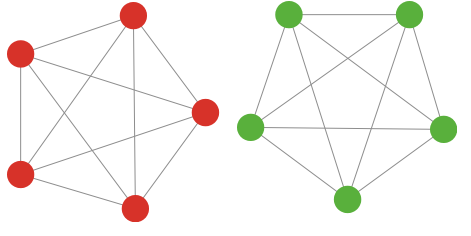
\includegraphics[scale=0.5]{../Figures/BonusGameInsuredClique.png}
  \caption{\label{fig:bonusoptimal} Two cliques, one consisting of insured agents the other consists of non-insured. All nodes have reached their goal. }
\end{figure}
As we see in Figure \ref{fig:bonusoptimal}, the results were as expected, the cost of insuring a link satisfied the conditions found earlier, and thus the result was two cliques, one consisting of only insured nodes and the other of non-insured nodes.
The price of anarchy in this scenario is 1, i.e. the socially optimal outcome. 

In the second simulation we set the parameter $m=5$, and kept the other variables unchanged. The resulting network was as expected the same as in the last simulation, but since the nodes did not reach their maximum degree, the price of anarchy is less than one. The price of anarchy can be seen in Eq.(\ref{eq:model-bonus-poa}).
\begin{eqnarray}
PoA&=\frac{\text{Sum of payoffs}}{\text{Sum of Socially optimal payoffs}}  \nonumber \\
PoA&=\frac{5\times 4\times (0.9-0.7)+5\times 4\times(0.9-0.5)}{5\times 4\times (0.9-0.7)+5\times 4\times(0.9-0.5)+5\times (2\times 0.9-0.7-0.5 + 2 \times 0.2)}\nonumber \\
PoA&=\frac{12}{17}
\label{eq:model-bonus-poa}
\end{eqnarray}

When we changed the link insurance cost to $I_{l}=0.5$, the resulting networks change. Now we found that the insured nodes are willing to establish risky links to reach their maximum degree. Some of the resulting networks can be seen in the figures \ref{fig:bonusvolating:a} and \ref{fig:bonusvolating:b}. In figure \ref{fig:bonusvolating:a} the price of anarchy is $0.95$, and in figure \ref{fig:bonusvolating:b} the price of anarchy is $1$, i.e. it has reached the socially optimal outcome.


\begin{figure}
  \centering
  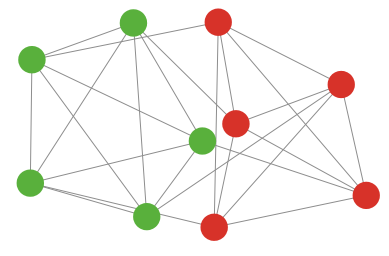
\includegraphics[scale=0.5]{../Figures/BonusGameViolatingOptimal.png}
  \caption{\label{fig:bonusvolating:b}Every non-insured node is connected to one insured node, this is the optimal outcome with these parameters.}
\end{figure}
  
\section{Model 2: Including bulk insurance discount}

 It seems to be common for insurance companies to offer discount to their customers if the customers choose to combine some or all of their insurances with them. We would like to introduce a discount rate dependent on the degree of the node. In a real-world scenario where nodes have an option of acquiring insurance or not, this will make it more attractive for nodes with high degree to acquire insurance, and the discount could act as an incentive for nodes to also acquire insurance. 

How insurance companies choose to formulate their discount rate might vary. One solution might be to follow a strict 5$\%$ discount per new connection, or let the discount follow a power law, or a log-function etc. We choose to follow a discount rule which directly reflects the node's degree.

\subsection{Analysis}
The price for adding a new link follows the equation:
\begin{equation}
\frac{I_{l}}{i+1}
\label{eq:discount0}
\end{equation}
Here, $i$ is the node's current degree. This means that the more links a node establishes the cheaper the link insurance will be. 

\subsubsection{Discount and Bonus model}

When the discount is applied to model 1, the only connection scenarios that is worth considering in this model is the ones where insured nodes connects to other insured nodes or when insured nodes connects to non-insured nodes.

When insured nodes are considering to establish links with eachother, their payoff functions are as shown in Eq.(\ref{eq:discount1}).  
\begin{equation}
    U_{i+1}= 
\begin{cases}
    \beta - I_{l},& \text{if } i = 0\\
    U_{i}+\beta -\frac{I_{l}}{i+1},& \text{if }  i>0\\
    U_{i}+\beta -\frac{I_{l}}{i+1}+\gamma,& \text{if } i=m-1
\end{cases}
\label{eq:discount1}
\end{equation}
For insured nodes to connect to eachother Eq.(\ref{eq:model4-bonus-i-to-i}) has to hold.

\begin{eqnarray}
U_{i}+\beta-\frac{I_{l}}{i+1}+\frac{\gamma}{m-i}&>U_{i} \nonumber \\ 
\beta-\frac{I_{l}}{i+1}+\frac{\gamma}{m-i}&>0 \nonumber \\ 
\llap{$\rightarrow$\hspace{50pt}}\beta +\frac{\gamma}{m-i}&>\frac{I_{l}}{i+1}
\label{eq:model4-bonus-i-to-i}
\end{eqnarray}

When insured nodes are considering to connect to non-insured nodes, their payoff functions are as shown in Eq. (\ref{eq:model4-bonus-i-to-ni}).
\begin{equation}
U_{i+1}= 
\begin{cases}
    \beta - I_{l}-r,& \text{if } i = 0\\
    U_{i}+\beta -\frac{I_{l}}{i+1}-r,& \text{if }  i>0\\
    U_{i}+\beta -\frac{I_{l}}{i+1}-r+\gamma,& \text{if } i=m-1
\end{cases}
\label{eq:model4-bonus-i-to-ni}
\end{equation}
For this to happen Eq.(\ref{eq:model4-bonus-i-to-ni-final}) has to hold.

\begin{eqnarray}
U_{i}+\beta-\frac{I_{l}}{i+1}+\frac{\gamma}{m-i}-r&>U_{i} \nonumber \\ 
\llap{$\rightarrow$\hspace{50pt}}\beta+\frac{\gamma}{m-i}&>r+\frac{I_{l}}{i+1}
\label{eq:model4-bonus-i-to-ni-final}
\end{eqnarray}

\subsection{Result and findings}

We want to find the condition for separating insured and non-insured nodes. The first step is to guarantee that insured nodes connect to eachother. To ensure that this happens, we need to find the condition for the lowest expected increase in payoff, i.e. at node degree zero. If nodes are willing to establish links at this point, then they will also be willing at all degrees higher than zero.
At degree zero there is no discount on the insurance link cost, and thus if Eq.(\ref{eq:conditionitoi}) from model 1 holds, insured nodes will connect to other insured nodes.

The condition for guaranteeing that insured nodes do not connect to non-insured nodes has changed, we know that if an insured node does not want to establish a link with a non-insured node at degree $m-1$, then neither will any insured node with degree lower than $m-1$ do so. From this we find the condition in Eq.(\ref{eq:model4-bonus-i-not-ni})
\begin{eqnarray}
U_{i}+\beta-\frac{I_{l}}{m}+\frac{\gamma}{m-(m-1)}-r&<U_{i} \nonumber \\ 
\beta+\gamma-r&<\frac{I_{l}}{m}\nonumber \\ 
\llap{$\rightarrow$\hspace{50pt}}m(\beta +\gamma-r)&<I_{l}\nonumber
\label{eq:model4-bonus-i-not-ni}
\end{eqnarray}
This is a very strong condition, because the only way this can happen is if $\beta+\gamma-r<\frac{1}{m}$.  This shows us that when the incentives for establishing links increase, it gets more and more difficult for the insurer to guarantee a clique of only insured nodes. 
The final condition for ensuring a clique of only insured nodes is shown in Eq.(\ref{eq:model4-final-condition-insured-clique}).

\begin{equation}
m(\beta +\gamma-r)<I_{l}<\beta+\frac{\gamma}{m}
\label{eq:model4-final-condition-insured-clique}
\end{equation}

The quantum discount results in an overall higher payoff for the insured nodes, since the cost of insuring a new link becomes cheaper. This means that the insured nodes will have a higher incentive to create links, making it harder for the insurer to separate insured and non-insured nodes.

We see that the problem of separating the two node types have increased compared to the previous model, meaning that if we have a network where the insurer has managed to separate them, the price of anarchy is also higher compared to a similar scenario in the first model. 

\section{Model 3: Network externalities}
In the earlier models when a node established a connection the change in utility were only dependent on fixed variables, and not dependent on the rest of the network. In many real world scenarios it is more realistic that a node will be strongly affected by the indirect connections to other nodes. Social relationships between nodes are good examples of such networks, where each person offer benefits in terms of favors, information etc. 

We apply the results from the paper from Jackson and Wolinsky \cite{jackson1996strategic} and use a network formation game found in \cite{jackson2005survey} to study indirect network effects in our model. 

The benefits a player receives in this game are calculated as follows: In addition to the benefit from the direct connection, a node will also benefit from "friends of the friend", and "friends of the friends of the friend" etc. This is achieved by letting the payoff be calculated relative to the distance between the nodes. $\beta$ now depends on the minimum number of hops to the node. We want the benefit to decrease with distance, therefore we need the limitation: $0<\beta<1$. 
The total payoff for a node is:

\begin{equation}
\sum_{j\neq i}^{} \beta_{ij}^{d(ij)} - \sum_{j:ij\in g}^{} {c}_{ij}, 
\label{eq:connecetionGame}
\end{equation}

Where $d(ij)$ represents the shortest path between node $i $ and node $j $, and ${c}_{ij}$ represents node i's cost of establishing a link between the two nodes. 

In the paper \cite{jackson1996strategic}, the authors analyze the networks created with these rules with two different approaches, one with focus on efficiency and the other on stability.  The optimal network is of course both efficient and stable, but as we shall see there are some conflicts between efficiency and stability. Matthew, et.al. showed that an efficient network is:
\begin{enumerate}
\item \textit{a complete graph $g^N$ if $c<\beta - \beta^2$,}
\item \textit{a star encompassing every node if $\beta - \beta^2 < c < \beta + \frac{(N-2)}{2}\beta^2$,}
\item \textit{an empty network (no links) if $\beta + \frac{(N-2)}{2}\beta^2 < c$.}
\end{enumerate}

The most efficient structure is a star structure which encompasses every node. A star structure has the characteristics of minimizing the average path length and uses the minimum number of links ($N-1$) required for including every node. However, it is not preferable to be the center node, due to the cost of all the direct links. 
This structure provides the highest overall payoff for the network, but this network is not necessarily stable.

When analyzing the stability of the network, by using the definition of pairwise stability, Jackson and Wolinsky found four different stability conditions:

\begin{enumerate}
\item \textit{a pairwise stable network consists of at most one (non-empty) component,}
\item \textit{if $c<\beta - \beta^2$, the unique pairwise stable network will be a complete graph $g^N$, }
\item \textit{if $\beta - \beta^2 <c < \beta $, a star encompassing every node will be pairwise stable, although not necessarily the unique pairwise stable graph,}
\item \textit{if $\beta < c$, any pairwise stable network which is nonempty is such that each player has at least two links and is thus inefficient. }
\end{enumerate}
We see that stability condition 2 is the same as efficiency condition 1, and therefore if this condition is fulfilled, the network is both stable and efficient. 
Condition 3 shows us why the efficient star network is not necessarily stable. If $\beta \leq c <   \beta + \frac{(N-2)}{2}\beta^2$ then the efficient network will be a star, but it is not stable.

It should be noticed that it is more beneficial for a node to operate as a leaf node compared to being a center node, due to the cost of direct connections.  

\subsection{Insurance and connection game}
The findings about efficiency and stability are very useful for our model, because if one has knowledge of the different variables it is possible to determine how the network will evolve. Additionally, if you are able to control the variables, you can actually determine the resulting network structure.

From this point on, the game we will consider is a homogeneous network setting, where every node is considered to be insured, and the benefit, $\beta$ and cost $I_{l}$ is the same for all nodes.
This is done because it will simplify an otherwise very complex model. 

In the paper \cite{jackson2005survey} the authors came up with the following proposition:
Consider the symmetric connections model in the case where $\beta-\beta^2<c<\beta$. As the number of nodes grows, the probability that a stable state (under the process where each link has an equal probability of being identified) is reached with the efficient network structure of a star goes to zero. But if a network reaches the efficient star structure, it is also pairwise stable, and will remain a star. 




Using the discount formula from the previous model, we end up with Eq.(\ref{eq:discountstar}) to achieve an efficient and stable star topology. $i$ represents the node degree.
\begin{equation}
\beta-\beta^2<\frac{i_{l}}{i+1}< \beta
\label{eq:discountstar}
\end{equation}
An interesting property when we include the discount is that the conditions for efficient and stable networks will change. Because
when the node degree increases, the insurance cost might reach the critical degree $g$, and the best strategy for a node with degree $g$ or higher, is to connect to every node, as shown in Eq.(\ref{eq:criticaldiscount}). The critical degree occurs when a node's optimal strategy changes from relaying on indirect connections to connecting to every node. 
\begin{equation}
\frac{I_{l}}{g}<\beta-\beta^2
\label{eq:criticaldiscount}
\end{equation}
This is possible when $g<n$, where $n$ represents the number of nodes in the network.
The stability condition has changed for a node with a critical degree. The stable and efficient condition for this node is, as shown earlier, to have a direct connection to every other node. Thus if we have a star topology, both the leaf nodes and the center node are stable, and the center node has been compensated for its role in the network. This could be used to increase the probability of reaching a star formation. 

When a node $i$ reaches the critical degree $g$ its optimal strategy is to connect to every node, since the payoff generated from direct connections is larger than any indirect connection. In general, nodes prefer to connect to nodes with high connectivity\footnote{A node with high degree implies a node with high connectivity.}, and will thus prefer to connect to this node compared to nodes with a degree lower than $g$. In this way, nodes will connect to the node who has a degree greater than or equal to $g$, and remove the links to their low-degree nodes which they can instead reach through the node with high connectivity.

From this we get the conjectures:
\begin{cnj}
If the critical degree ratio is low, i.e. the ratio between critical degree and number of nodes in the network, the resulting network will with high probability be a clique.
\label{prop:clique}
\end{cnj} 

\begin{cnj}
If the critical degree ratio is at a medium level, the resulting network will with high probability be a star. 
\label{prop:star}
\end{cnj}

\begin{cnj}
If the critical degree ratio is high, the resulting network will with high probability be a star-like/scale-free structure. 
\label{prop:scale-free}
\end{cnj}

A numerical example of the boundaries between the different structures, we found from our simulation (described in the next section) with 20 nodes is the following: 
As seen in Figure \ref{fig:PlotStar} a critical degree of 1-5 applies to conjecture \ref{prop:clique}, 6-12 applies to conjecture \ref{prop:star} and 13-20 applies to conjecture \ref{prop:scale-free}. 

\subsubsection{Results and findings}

To prove the conjectures above, we created a simulator. The rules of the simulator are as following:
Every round of the game,two random nodes, not neighbors, are selected, and asked if they would want to establish a link. The link establishment is a symmetric decision, i.e. the link is established if it result in an increased payoff for both nodes. If the link is added, we check if either of the nodes would prefer to delete some of their already existing links, this decision is asymmetric. A link will be deleted if the node will achieve a higher payoff without it. Then we ask the rest of the nodes if they would like to delete any links. This procedure is repeated as long as it is possible to add new links. 
The payoff function of each node is as described earlier (see Eq.(\ref{eq:connecetionGame})), except that the cost is now dependent on the degree of the node. For the simulations to be realizable, we had to set the number of nodes to 20, or else the computational time would be to high. For every critical degree, from three to nineteen, we ran 50 simulations, and noted the resulting network formation. We chose to start from critical degree equal three, since any number below would result in a clique, because it would be more beneficial to be directly connected to every node.  

We know that if Eq.(\ref{eq:discountstar}) is satisfied for all $i$, then the efficient and stable state is a star. But a more interesting scenario occurs when we have a graph where one or more of the nodes reaches the critical degree. -Will the final structure be scale-free, a star or simply just unstructured? 
The results from the simulation can be seen in Figure \ref{fig:PlotStar}, \ref{fig:PlotClique} and \ref{fig:PlotStarIsj}. As we see from Figure \ref{fig:PlotStar}, the probability of the resulting network being a star suddenly increases from zero to 42\% at critical degree five to six, and then jumps from 42 to 70-, 86-,96-, 98\% at critical degree six to nine. These results confirm our conjectures, and show that the discount can drastically increase the probability of the network ending up in a star. 

\begin{figure}
\centering
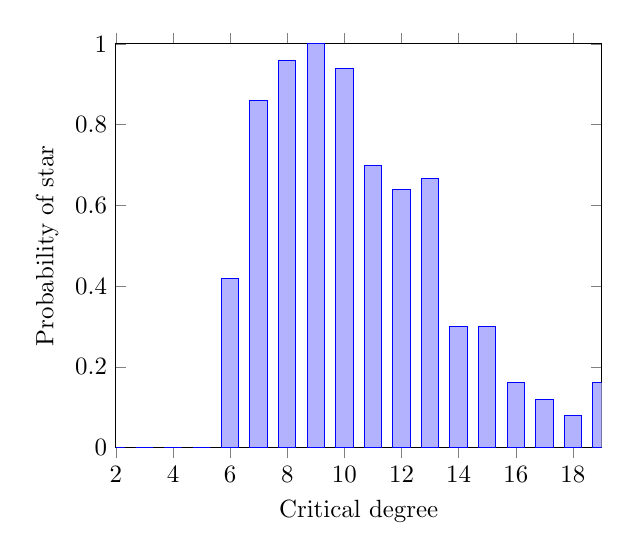
\begin{tikzpicture}[thick,scale=0.9]
\begin{axis}[
x tick label style={
	/pgf/number format/1000 sep=},
	ylabel=Probability of star,
	xlabel=Critical degree,
enlargelimits=0.0,
legend style={at={(0.5,-0.15)},
anchor=north,legend columns=-1},
ybar,
bar width=7pt,
]
\addplot
coordinates {
(2,0.0) (3,0.0) (4,0.0) (5,0.0) (6,0.42) (7,0.86) 
(8,0.96) (9,1.0) (10,0.94) (11,0.70) (12,0.64)
 (13,0.667) (14,0.3) (15,0.3) 
(16,0.16) (17,0.12) (18,0.08) (19,0.16) };
\end{axis}
\end{tikzpicture}
\caption{\label{fig:PlotStar} Shows the probability of the network ending up in a star, given different critical degrees.}
\end{figure}

From Figure \ref{fig:PlotClique} we can observe that the opposite is happening when the critical degree is increased; the probability of the resulting network being a clique drastically decreases. As we can see with a critical degree of seven or higher, it is very unlikely that we end up with a clique. These findings support our conjectures.

\begin{figure}
\centering
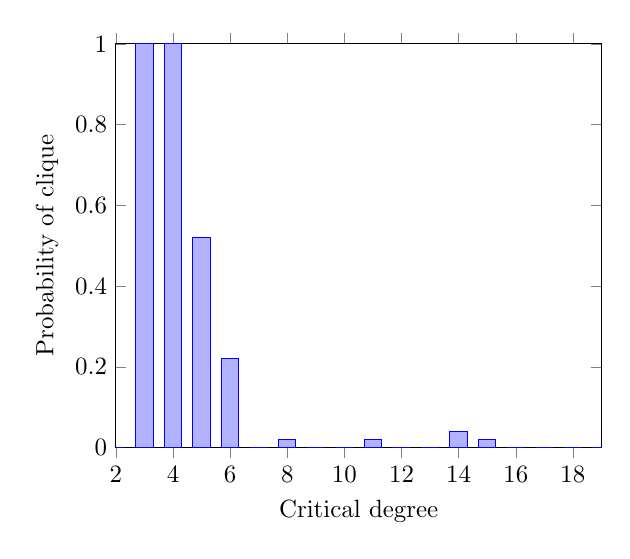
\begin{tikzpicture}[thick,scale=0.9]
\begin{axis}[
x tick label style={
	/pgf/number format/1000 sep=},
	ylabel=Probability of clique,
	xlabel=Critical degree,
enlargelimits=0.0,
legend style={at={(0.5,-0.15)},
anchor=north,legend columns=-1},
ybar,
bar width=7pt,
]
\addplot
coordinates {
(2,0.0)(3,1.0) (4,1.0) (5,0.52) (6,0.22) (7,0.0) 
(8,0.02) (9,0.0) (10,0.00) (11,0.02) (12,0.0)
 (13,0.0) (14,0.04) (15,0.02) 
(16,0.0) (17,0.0) (18,0.00) (19,0.0) };
\end{axis}
\end{tikzpicture}
\caption{\label{fig:PlotClique} Shows the probability of the network ending up in a clique, given different critical degrees.}
\end{figure}

In Figure \ref{fig:PlotStar} when the critical degree gets closer to the number of nodes in the network, the probability of the network evolving into a star decreases. However, in Figure \ref{fig:PlotStarIsj}, we have plotted the probability of the network evolving into a network where only a few(2-4) nodes end up with a high degree, but not necessarily a critical degree. As we see, this occurs with high probability from critical degree six and up. These networks are so called scale-free networks (A-B graphs, described in the methodology chapter), because there are a few hubs, that account for most of the connectivity in the network. The reason why we end up with a scale-free network is because nodes prefer to be connected with nodes with high connectivity, and thus will delete links to nodes with low connectivity. This is very similar to the simple model that creates scale-free networks, where the probability of connecting to a node is proportional to the degree of the node.


\begin{figure}
\centering
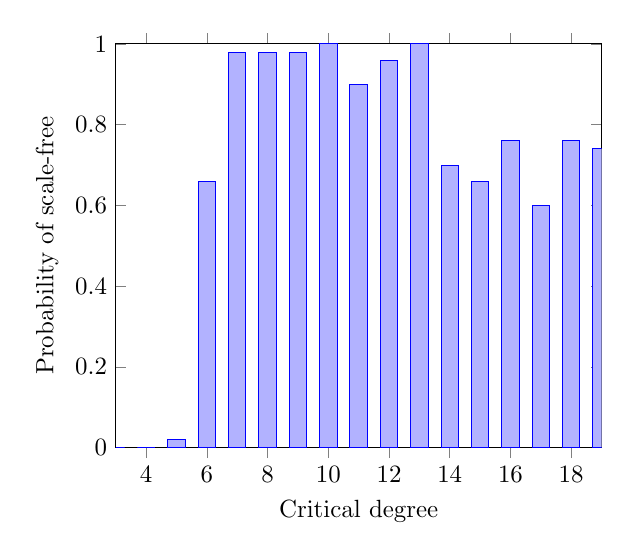
\begin{tikzpicture}[thick,scale=0.9]
\begin{axis}[
x tick label style={
	/pgf/number format/1000 sep=},
	ylabel=Probability of scale-free,
	xlabel=Critical degree,
enlargelimits=0.0,
legend style={at={(0.5,-0.15)},
anchor=north,legend columns=-1},
ybar,
bar width=7pt,
]
\addplot
coordinates {
(3,0.0) (4,0.0) (5,0.02) (6,0.66) (7,0.98) 
(8,0.98) (9,0.98) (10,1.00) (11,0.90) (12,0.96)
 (13,1) (14,0.7) (15,0.66) 
(16,0.76) (17,0.60) (18,0.76) (19,0.74) };
\end{axis}
\end{tikzpicture}
\caption{\label{fig:PlotStarIsj} Shows the probability of the network ending up in a scale-free structure, given different critical degrees.}
\end{figure}
\paragraph{Price of Anarchy.}
Another interesting thing is the average price of anarchy as function of the critical degree. The price of anarchy was calculated by taking the average total payoffs and dividing on the optimal payoff. The result can be seen in Figure \ref{fig:plotpriceofanarchy}. 

We see that the price of anarchy for the first critical degrees is 1, and then decreases until degree six, and at seven it increases again. This is because at degree one to five, the socially optimal structure is a clique. At degree six, a clique and a star, are almost equally good, and at degree seven and up, a star structure is the socially optimal outcome. 
In other words, when the cost is low, a clique is the optimal structure, and when the cost is high a star is the optimal structure. 

This further improves our findings, because we have now shown how an insurer can determine the resulting network formation by changing the cost. In addition, the formation that evolves has a price of anarchy close to 1. 

\begin{figure}
\centering
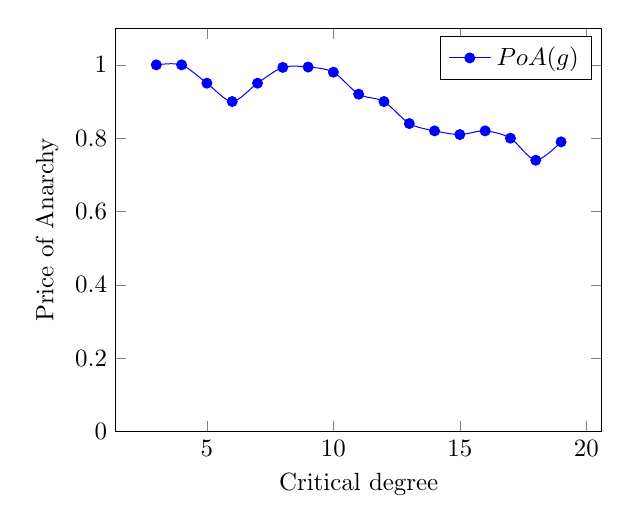
\begin{tikzpicture}[thick,scale=0.9]
\begin{axis}[
	ylabel=Price of Anarchy,
	ymin=0.0,
	xlabel=Critical degree]
\addplot [smooth,mark=*,blue] plot coordinates {

(3,1) (4,1) (5,0.95) (6,0.9) (7,0.95) 
(8,0.993) (9,0.994) (10,0.98) (11,0.92) (12,0.90)
 (13,0.84) (14,0.82) (15,0.81) 
(16,0.82) (17,0.8) (18,0.74) (19,0.79) };
\addlegendentry{$PoA(g)$}
\end{axis}
\end{tikzpicture}
\caption{\label{fig:plotpriceofanarchy} Shows the price of anarchy as a function of critical degree}
\end{figure}






\section{Discussion}
\section{Discussion}
In this paper we have introduced tree different models of endogenous network formation. The first model can be applied to certain real-world scenarios, such as software development firms/chains, or other networks where the final product is dependent on the collaboration of multiple participants.
This was done by letting node get a bonus, which is first received when a node reaches the desired number of links (called max-degree). This made the separation process of insured and non-insured nodes difficult for the insurer. Due to the possibility of achieving the bonus, a node will have a high incentive to establish links, and is thus more accepting towards establishing links with risky nodes, compared to a scenario without bonus. The conditions for separating insured and non-insured nodes in this model are: $\beta+\gamma-r<I_{l}<\beta+\frac{\gamma}{m}$. For the separation of insured and non-insured nodes to be possible, the following has to hold: $1-\frac{1}{m}<\frac{r}{m}$. As we see, as $\gamma$ and/or $m$ increases, this gets more and more difficult to achieve. 

In Model 2 we tried to implement a common feature used by insurance companies, bulk discount, in order to see how this affected the network formation. The cost of insuring a link is now dependent on the node's degree. 
The discount resulted in higher incentive for insured nodes to establish links with non-insured nodes. The reason is intuitive, since the cost of doing so decreases as the node degree increases. 
The condition to ensure separation becomes: $m(\beta+\gamma-r)<I_{l}<\beta+\frac{\gamma}{m}$, it is now harder for the insurer to separate the insured and non-insured from eachother. 

To ensure separation the insurer has to set a higher price to compensate for the increased incentive of link establishment, therefore the potential price of anarchy is higher than in model 1.

In our last model we applied the discount to an already existing model, "the symmetric connection game". In this old game it has been shown that there are three different efficient and stable networks, clique, star and an empty network, that arise under certain cost conditions. If $I_{l}<\beta-\beta^{2}$, the efficient and stable network is a clique. If $\beta-\beta^{2}<I_{l}<\beta$ a star is both stable and efficient. If $I_{l}>\beta+\frac{N-2}{2}\beta^{2}$ an empty network is both stable and efficient. In general, a clique is the most efficient if the cost of establishing links is less than the benefit gained from indirect connections. A star is the most efficient if the cost is higher than the benefit from indirect connections, but less than the benefit of direct connections. 
However, it is proved that as the number of nodes in the networks increases, the probability of the network ending up in star goes to zero. But, when we applied our insurance discount to this model, we found conjectures saying that, by setting the cost to the right level, one can with high probability ensure that either a clique, a star or a scale-free structure will evolve. This changes the connection game drastically, because now the insurer is able to force the network into three possible network formations, where the star has a fixation probability that exceeds the cliques. The insurer can use these findings to ensure that one of the beneficial structures, star or clique evolves. If the insurer is able to force a star to evolve, this can be used to drastically increase the overall security, and at the same time minimize the overall link cost. 

\section{Conclusion}
From our background study, it was revealed that the current market for cyber-insurance is far from healthy, and many have failed in attempts to establish a cyber-insurance market.
As described in the introduction, there are certain obstacles that are unique for cyber-insurance, and arguably these are the reasons why cyber-insurance has not emerged as expected. 
 However, we believe that there is a need for cyber-insurance, and that our new approach of analyzing the cyber-insurance market through graphs and network formation games could help establishing and improving the market.

We studied a variety of different network formation games, in order to find out if there were any superior network topologies that would fit as a cyber-insurance network, were ideally both the insurer and customers get a higher payoff from purchasing cyber-insurance. 
We found that star and clique networks had appropriate characteristics, not only do they have calculable fixation probability, but they could also generate better security and overall higher payoff for the nodes. With these networks in mind, we wanted to find a way of forcing networks to evolve into these structures.  We found that insurers could adjust the insurance premium in order to control the formation of networks. If the price is set to the right level, networks with calculable risk will evolve, and if the insurer is able to separate the nodes into two different networks, one consisting of trusted, insured nodes, the other of non-insured nodes, the trusted nodes can even further increase their payoff, compared to a non-trusted network. The insurer now possesses a tool for setting the insurance premium properly, possible resulting in better products for both the customer and the insurer.

\paragraph{Limitations and future work}
One limitation to our work, and a suggestion for future work, is to map our models and simulations to real-world networks in a more convincing way. Real-world networks are not random. Nodes may prefer to talk to nodes with high degree or low degree. In addition, the decision to use additive risk were taken due to the simplicity of the function and the fact that we do not know how a real-world risk distribution actually looks like.  By introducing a complex risk function, we would only have distorted the goal of our models. i.e. suggestions for improving our models is to introduce more realistic payoff functions.

%
\begin{thebibliography}{[MT1]}
%
\bibitem[CE1]{clar:eke}
Clarke, F., Ekeland, I.:
Nonlinear oscillations and
boundary-value problems for Hamiltonian systems.
Arch. Rat. Mech. Anal. {\bfseries 78} (1982) 315--333
%
\bibitem[CE2]{clar:eke:2}
Clarke, F., Ekeland, I.:
Solutions p\'{e}riodiques, du
p\'{e}riode donn\'{e}e, des \'{e}quations hamiltoniennes.
Note CRAS Paris {\bfseries 287} (1978) 1013--1015
%
\bibitem[MT1]{mich:tar}
Michalek, R., Tarantello, G.:
Subharmonic solutions with prescribed minimal
period for nonautonomous Hamiltonian systems.
J. Diff. Eq. {\bfseries 72} (1988) 28--55
%
\bibitem[Ta1]{tar}
Tarantello, G.:
Subharmonic solutions for Hamiltonian
systems via a $\bbbz_{p}$ pseudoindex theory.
Annali di Matematica Pura (to appear)
%
\bibitem[Ra1]{rab}
Rabinowitz, P.:
On subharmonic solutions of a Hamiltonian system.
Comm. Pure Appl. Math. {\bfseries 33} (1980) 609--633
\end{thebibliography}
%

\end{document}
